%% This document gives an example on how to use the ntnumasterthesis
%% LaTeX document class.

%% Use short name MACS, MIS, CIMET, MTDMT, MIXD or MIS  
%% Language english or norsk
%% b5paper with oneside or twoside, you can set A4 if you want but you submit in b5

%% If you want print with the heading material on a4 paper you can use this format
%% \documentclass[MACS,english,a4paper,oneside,12pt]{ntnuthesis/ntnuthesis}

%% with the change to using DAIM we have a new option. include DAIM after english below removes the front page material so that you can then submit in the DAIM system. If you are wanting the front material remove DAIM and make sure you fill in the DaimData.tex file.
\documentclass[MACS,english]{ntnuthesis/ntnuthesis}

\usepackage[T1]{fontenc}
\usepackage[utf8]{inputenc}     % For utf8 encoded .tex files allows norwegian characters in the files. This can be dangerous if you change to a differnt editor.
%\usepackage[pdftex]{graphicx, hyperref}   % For cross references in pdf
\usepackage{graphicx}
\usepackage{hyperref}   % For cross references in pdf


\usepackage{color}              % For colouring text 
\hypersetup{colorlinks=true,     
		linkcolor=blue,          % color of internal links (change box color with linkbordercolor)
    citecolor=blue,        % color of links to bibliography
    filecolor=blue,      % color of file links
    urlcolor=blue           % color of external links
		}
\usepackage{csvsimple}  % for simple table reading and display
\usepackage{url}
\usepackage{booktabs}
\usepackage{gnuplottex} %miktex option if using miktex on windows
\usepackage{rotating}


\definecolor{darkgreen}{rgb}{0,0.5,0}
\definecolor{darkred}{rgb}{0.5,0.0,0}

\lstset{        basicstyle=\ttfamily,
                keywordstyle=\color{blue}\ttfamily,
                stringstyle=\color{darkred}\ttfamily,
                commentstyle=\color{darkgreen}\ttfamily,
}


%Typesetting of C++ but not always stable in titles etc...
\newcommand{\CPP}[0]{{C\nolinebreak[4]\hspace{-.1em}\raisebox{.1ex}{\small\bf +\hspace{-.1em}+\ }}}

%\usepackage[table]{xcolor}% http://ctan.org/pkg/xcolor
%\usepackage[nomessages]{fp}
%\newlength{\maxbarlen}


\newcommand\databar[3][gray!20]{%
  \FPeval\result{round(#3/#2:4)}%
  \rlap{\textcolor{#1}{\hspace*{\dimexpr-\tabcolsep+.5\arrayrulewidth}%
        \rule[-.05\ht\strutbox]{\result\maxbarlen}{.95\ht\strutbox}}}%
  \makebox[\dimexpr\maxbarlen-2\tabcolsep+\arrayrulewidth][r]{#3}}



\newcommand{\com}[1]{{\color{red}#1}} % supervisor comment
%\renewcommand{\com}[1]{} %remove starting % to remove supervisor comments
% This will appear in text \com{Lecuters comment} and be visible unless you uncomment
% the renewcommand line.

\newcommand{\todo}[1]{{\color{green}#1}} % items to do
%\renewcommand{\todo}[1]{} %remove starting % to remove items to do

\newcommand{\n}[1]{{\color{blue}#1}} % other comment
%\renewcommand{\n}[1]{} %remove starting % to remove notes

\newcommand{\dn}[1]{} % add the d to a note to say that you have finished with it.





% Set to true ONLY if using Harvard citation style
\newboolean{HarvardCitations}
\setboolean{HarvardCitations}{false} % false for computer science, true for interaction design and harvard style


\ifthenelse{\boolean{HarvardCitations}}{%
	\usepackage{natbib} % for Harvard names as citations.
}{%
	\usepackage[numbers]{natbib} % for Vancover numbers in bibliography
}

\newcommand{\q}[1]{\leavevmode\marginpar{\small\em #1}}
\renewcommand{\q}[1]{}


\begin{document}

% for students submitting in the DAIM system this information will not be used.
% their is an option for DAIM submission which removes this information and checks it is B5.
% Removing the DAIM option on the document type will use this material.

\setthesistitle{User-centred Chatbot Personalities: a stable pattern for a more effective design processes of conversational interfaces}
\setthesisshorttitle{User-centred chatbot personalities} % a short version for the page headers if your normal title is too long to fit
\setthesisauthor{Tuva Lunde Smestad}
\setthesissupervisor{Frode Volden}
\setthesissupervisorA{Anders-Petter Andersson}  % if you have a second supervisor add it like this
%\setthesissupervisorB{Prof. Smart Guy}  % if you have a second supervisor add it like this


\nmtkeywords{Personality, Chatbot, Conversational Interfaces, Thesis, User Centred Design, User Experience, Personality, Character Development}
%\nmtdesc{This is the short description of a masters thesis}


\setthesisdate{01-06-2018}
\setthesisyear{2018}



%for CIMET theses you need to see all of these as well

%\setthesiscampus{Gj\o{}vik}
%\setthesisHostInstitution{\NTNU}
%\setthesisHostInstitution{University of Eastern Finland}
%\setthesisHostInstitution{Universit\'e Jean Monnet Saint-Etienne}

%\setthesisjuryA{} %jury names
%\setthesisjuryB{} %jury names
%\setthesisjuryC{} %jury names
%\setthesisjuryD{} %jury names


 % this is the file which contains all the details about your thesis
\makefrontpages % make the frontpages
%this is the intro to the thesis
%\thesistitlepage % make the ordinary titlepage
\hypersetup{pageanchor=false}
%\include{summary}

\chapter*{Preface}
This master thesis is the final part of my Master in Interaction Design degree at the department of Design at the Norwegian University of Science and Technology (NTNU). The project planning and preliminary studies/literature review was conducted during the autumn of 2017. The work presented in this thesis was conducted and written during the spring of 2018 and the workload corresponds to 30 ECTS.

Throughout my work as an interaction designer I was challenged with building my first chatbot and was surprised to find that much work is still to be done regarding the user experience of chatbots. Most of the frameworks acts more like "do's" and "dont's" rather than based on research. And a lot of these guidelines are based on assumptions, or small case studies that do not necessarily extends to the larger application of conversational agents. Not wanting chatbots to be abandoned early by users because the implementation of these systems are far behind the technological development, I set out with this thesis to try and prove at least one assumption: does personality improve the user experience of chatbots?

I aim with this master thesis to add to the field of human-computer and human-robot interaction by providing evidence to explain how personality impacts the user experience of machines that can converse. In addition to this I'm also providing other designers and developers, interested in conversational interfaces, with a framework to build synthetic personalities for chatbot agents.

This thesis is for anyone who wishes to design their own chatbot with a basis in personality, and those who like me are eager to determine how we can improve the user experience of conversational interfaces.

\vspace{5mm}

%\begin{center}
%\thesiscampus, 
\thesisdate \\[1pc]
\\[1pc]
%\thesisauthor
%\end{center}

\chapter*{Acknowledgment}
I would like to thank the following persons for their great help during the course of this thesis project:

\vspace{5mm}

My partner Christopher Solem for providing emotional support, extraordinary listening skills, helpful commentary and for proof reading not only my thesis, but the literature review and project planning report. I would not have survived my masters degree without you.

\vspace{5mm}

Mom and dad for their long standing support, both emotional and material, and for lending me your car so I could get around to all who participated in my experiment.

\vspace{5mm}

The participants for taking time out of their busy schedule to help me with my thesis project.

\vspace{5mm}

My supervisor Frode Volden, for keeping my research aim on track, reminding me to not forget about the overall aim and not become too concerned about the design and building of the chatbot prototype. I am grateful for all your help and your sound knowledge in SPSS, which I would not have made it without!

\vspace{5mm}

My co-supervisor Anders-Petter Andersson for providing challenging questions that made me stop to reassess and question my choices throughout the process. Pointing me in the direction of valuable resources and articles, designs and research to help me get a thorough understanding of the field I now have explored.

\begin{flushright}
T.L.S.\\[1pc]
\end{flushright}

\include{Abstract}



\tableofcontents

\hypersetup{pageanchor=true}

% Comment with a percent to remove figures or tables:
\listoffigures
\listoftables


\chapter{Introduction}
\label{chap:introduction}
\q{What is the purpose of this document?}
The purpose of the current document is to provide an example of using the thesis template and a description on how to use \LaTeX. There are instructions that relate specifically to the template, and some which are generally useful for \LaTeX. 

\q{Where is the structure defined } 
The detailed typographical rules have been implemented in the
\texttt{ntnuthesis} \LaTeX\ document class, in the file 

This was updated by Simon McCallum.
The package has changed names and version number it is now called
\texttt{ntnuthesis}
v\ntnuthesisversion\ as of \ntnuthesisdate.

\q{what is a thesis about}
For many of you, this Master's thesis will be the most advanced academic document you ever write.  It needs to demonstrate both academic ability and clear thinking. You Master's should show that you are ready to lead other people, reflect more deeply, and have a professional attitude to your work and environment. 

\q{who cares}
When writing the thesis it is important to know who you are writing for. The target audience for this document is in layers:
\begin{enumerate}
    \item The marking committee
    \item Your supervisor
    \item Other students at the same level 
    \item Professionals \& Academics
    \item The general public.
\end{enumerate}

\section{Problem Description}
The chatbots of 2017 have not truly improved since the first chatbot ELIZA back in 1966. While the programming behind conversational interfaces are fast improving, making use of Artificial Intelligence (AI) and Natural Language Processing (NLP), a chatbot is still a form of weak-AI in which makes use of stimulus-response approach. Human interaction and conversation consists of a lot more than predicting user intentions, analyse keywords to define meaning, and then respond from a predefined set of responses. Therefore, no matter how accurate the chatbot is in predicting what humans actually mean, and how well it performs its tasks, they are not perceived as intelligent conversational entities. Predictions and recent research find chatbots to be a big part of an AI powered future, but recent reviews of chatbots have found them to be unintelligent and non-conversational (Stokke, 2017, Orf, 2017, Piltch, 2017, Vincent, 2017, Boutin, 2017). Piltch (2017) states that we should not be carried away by the positive outlook researchers presents in regards to the possibilities of advances in AI technology for chatbot technology, as the reality is that most chatbots are falling flat. Despite cautions and recent negative reviews, Forrester (2017) found that 56 \% of companies have implemented or are planning to implement a chatbot as part of the services they provide in the near future. JuniperResearch (2017) released a report in which they have found that chatbots will save companies \textdollar 8 billion in costs by 2022. Therefore, as the trends predict many benefits for companies implementing chatbots, are we forcing users to adopt technology which they find frustrating and useless? If the reviews find chatbot interactions as unintelligent, pointless, and not more effective than conducting a Google search or contacting a human customer service agent, what effects might this have on the user experience?

\section{Justification, Motivation and Benefits}
Ever since ELIZA, the goal of chatbot systems have been to pass the Turing Test, and convince humans that they are conversing with a human, not a machine \citep{McTear2016b}. However, available chatbots does not appear to possess human conversational skills, rather they perform as a machine by responding to user commands. This shows that although a chatbot is more flexible in regards to it being able to understand vast variations of the same command, it still functions as a command-based system. To be perceived as conversational agents, chatbots needs to be able to do a lot more than input-output. Therefore, understanding why chatbots are failing to be conversational and what we can do to allow users to perceive them as more than a computer, can have a great impact on improving the user experience. To understand how we can design chatbots that are perceived as more conversational, means that we must take into account many other factors of human interaction beyond only language understanding. Humans have bodies, feelings, emotions, different personalities and behaviours that all influence how we communicate, behave, and interact. Humans are extremely skilled social actors, and in order to design chatbots that too are skilled social actors we must understand the social cues that make up human interaction, and the personalities that drives them. 

This master thesis project will explore how we can build chatbots that offer a better user experience and are perceived as more conversational through focusing on the design of chatbot personalities. The thesis will understand how thinking about the chatbot as a character with a mind of its own, can benefit the design process and result in more conversational and improved user experience. In addition to this, chatbots are extensions of services provided by companies, therefore it is also important to design personalities that reflects the brand it represents. Through this topic the researcher hopes to add to the understanding of how designers can create better chatbot interfaces, and offer a framework to inform how designing chatbot personalities can benefit the design process as a whole. As trends show that companies are rapidly implementing chatbots as part of their services, consumers should not be forced to adopt solutions that does not improve the effectiveness, efficiency or satisfaction. This investigation would also benefit companies, as this knowledge can help ensure improved services for their customers, and consistent communication in its tone of voice through the chatbot.

\section{Research Questions}
The research questions and sub-questions to be addressed in the master thesis project are:

\begin{enumerate}
    \item How can we design chatbot personalities to guide the design process of a chatbot interface and create a better user experience?
    \subitem a) Which elements must be considered to inform a chatbot personality?
    \subitem b) What components needs to be in place for a chatbot personality to meet user needs and expectations?
    \item How can personality be used as a design variable to allow users to perceive chatbots as more than a computer?
        \subitem a) How can designers use personality to improve the conversational design of chatbots?
        \subitem b) How will the personality affect the user experience?
        \end{enumerate}

\section{Planned Contributions}
The results from exploring techniques to design user-centred chatbot personalities will be presented to define a UX framework that designers can use to build user centred chatbot personalities. This master thesis will produce a framework that entails different methods and techniques that designers can use to design a chatbot persona that meets user needs and is consistent with the brand's tone of voice. This framework will form a foundation to guide the design process of chatbots, towards improved user experience. This framework will inform what elements that needs to be considered to inform the type of personality that is appropriate, and which methods that could help design the personality to be in line with users' needs as well as the brand it represents. This framework will also inform how the chatbot personality can be used to guide and inform other aspects of the design of chatbots such as the conversation design. The framework will include methods to not only design, but evaluate design decisions in relation to the user experience, show how companies can extend and add value to their brands by providing a chatbot experience that is consistent with the brand's tone of voice. % includes latex files from the same directory
\chapter{Packages}
\label{chap:packages}

The \texttt{ntnuthesis} is built upon the standard \LaTeX\
\texttt{report} class. All commands from the \texttt{report} class can
be used, with the two exceptions of \verb+\subsubsection+ and
\verb+\paragraph+. This is because there should only be three
levels of headings according to the guidelines. 
It has been placed in a folder called \texttt{ntnuthesis} so that it does not
clutter your work.  You should not change anything in \texttt{ntnuthesis}. If you need to change 
anything you should make a pull request on the github repository for this thesis at
\url{https://github.com/COPCSE-NTNU/master-theses-NTNU}

\section{Packages Used by ntnuthesis}
\label{sec:packages}

In addition to the \texttt{report} document class,
\texttt{ntnuthesis} makes direct use of the following packages
that must hence be present:
\begin{description}
	\item[geometry:] used for setting the sizes of the margins and
  	headers.
	\item[fontenc:] used with option \texttt{T1} for forcing the Cork font
  	encoding (necessary for the Charter font).
	\item[charter:] load Charter as the default font.
	\item[euler:] load the Euler math fonts.
	\item[bable:] for language handling.
	\item[listing:] for code listing.
\end{description}

\section{Other Relevant Packages}
\label{sec:otherpackages}

The author of a thesis might want to use a bunch of different packages
to those described in Section~\ref{sec:packages} in order to have all features needed for their document. 
In particular, it is advised to use the following:
\begin{description}
	\item[inputenc:] to allow \LaTeX\ to use more than 7-bit ASCII for its
	  input. Most often, the option \texttt{latin1} will do.
	\item[babel:] to load language specific strings. Reasonable options
	  include \texttt{british}, 
		\texttt{american}, \texttt{norsk} and
	  \texttt{nynorsk}.
	\item[graphicx:] to include graphics.
	\item[hyperref:] this is a very nice package that makes cross links in
	  pdf documents. Use with option \texttt{dvips} or \texttt{pdftex}
	  in accordance with the driver that you use. Unfortunately, hyperref
	  is not completely bugfree\dots
\end{description}

We have web pages as well~\cite{NTNU:Website}, and now games like Halo~\cite{Halo}. % could be called Methodology or methods or any filename 
\chapter{Structural Elements}
\label{chap:structural}

If you are submitting using the DAIM system you should make sure the pdf you submit does not have the front page information, as that will be added by the submission form in DAIM.  You can remove the DAIM option to print the front page material if you want a full PDF with the front page material. To make sure the running header has the title of the thesis you still need to set it in the \verb+DaimData.tex+ file. The title of the thesis should be set using the \verb+\thesistitle+
command, and the date of the thesis should be set using the
\verb+\thesisdate+ command in the \verb+DaimData.tex+ file. 

\section{Page Layout}

The geometry of the page has been set using the \verb+\geometry+
command.

\section{Fonts}

Due to limited \LaTeX\ support for the Georgia font, Charter has been
chosen instead. For mathematical formula, the Euler fonts are used,
since they blend more nicely with the Charter than the standard
\LaTeX\ fonts: 
\begin{equation} \label{eq:1}
    f(x) = \int_0^x g(\tau)\,d\tau
\end{equation}



For inline math you can use $\backslash{}($ and $\backslash{})$ for example \( f(x)= \frac{x^2}{1+x^2} \).  
This also allows you to use $\slash$ and $\backslash$. You need to include the \{\} when you want the special
character to have other letters immediately after it.

\section{Sectioning Commands}

The standard \LaTeX\ sectioning commands are used for both numbered
and unnumbered sections. The top level is given by the \verb+\chapter+
command. This starts a new right page. The two lower levels are
obtained using the \verb+\section+ and \verb+\subsection+ commands.
The standard \LaTeX\ \verb+\subsubsection+ and \verb+\paragraph+
commands have been disabled since their use is not encouraged by the
thesis guidelines. When you use these they will not be given numbers.  
They still appear in the document with highlighting but not in the 
table of contents.

\subsection{The subsection}

This is an example of a subsection.

\subsubsection{The subsubsection}

This is an example of a subsubsection.

\paragraph{The paragraph}

This is an example of a paragraph with a heading.

\section{Floats (Figures and Tables)}
\label{sec:floats}

Figures are placed in the \texttt{figure} environment. An example is
shown in Figure~\ref{fig:example}. %notice the ~ in between figure and the \ref. it stops latex from splitting the number and word over a line.
Tables are placed in the \texttt{table} environment. An example is given in
Table~\ref{tab:example} and reading the information directly from file in Table~\ref{tab:examplecsv}. Figures and tables float freely around in the
document in accordance with standard \LaTeX\ behavior.

\begin{figure}[tbp]  %t top, b bottom, p page | you can also use h to try to get the figure to appear at the current location
  \centering
  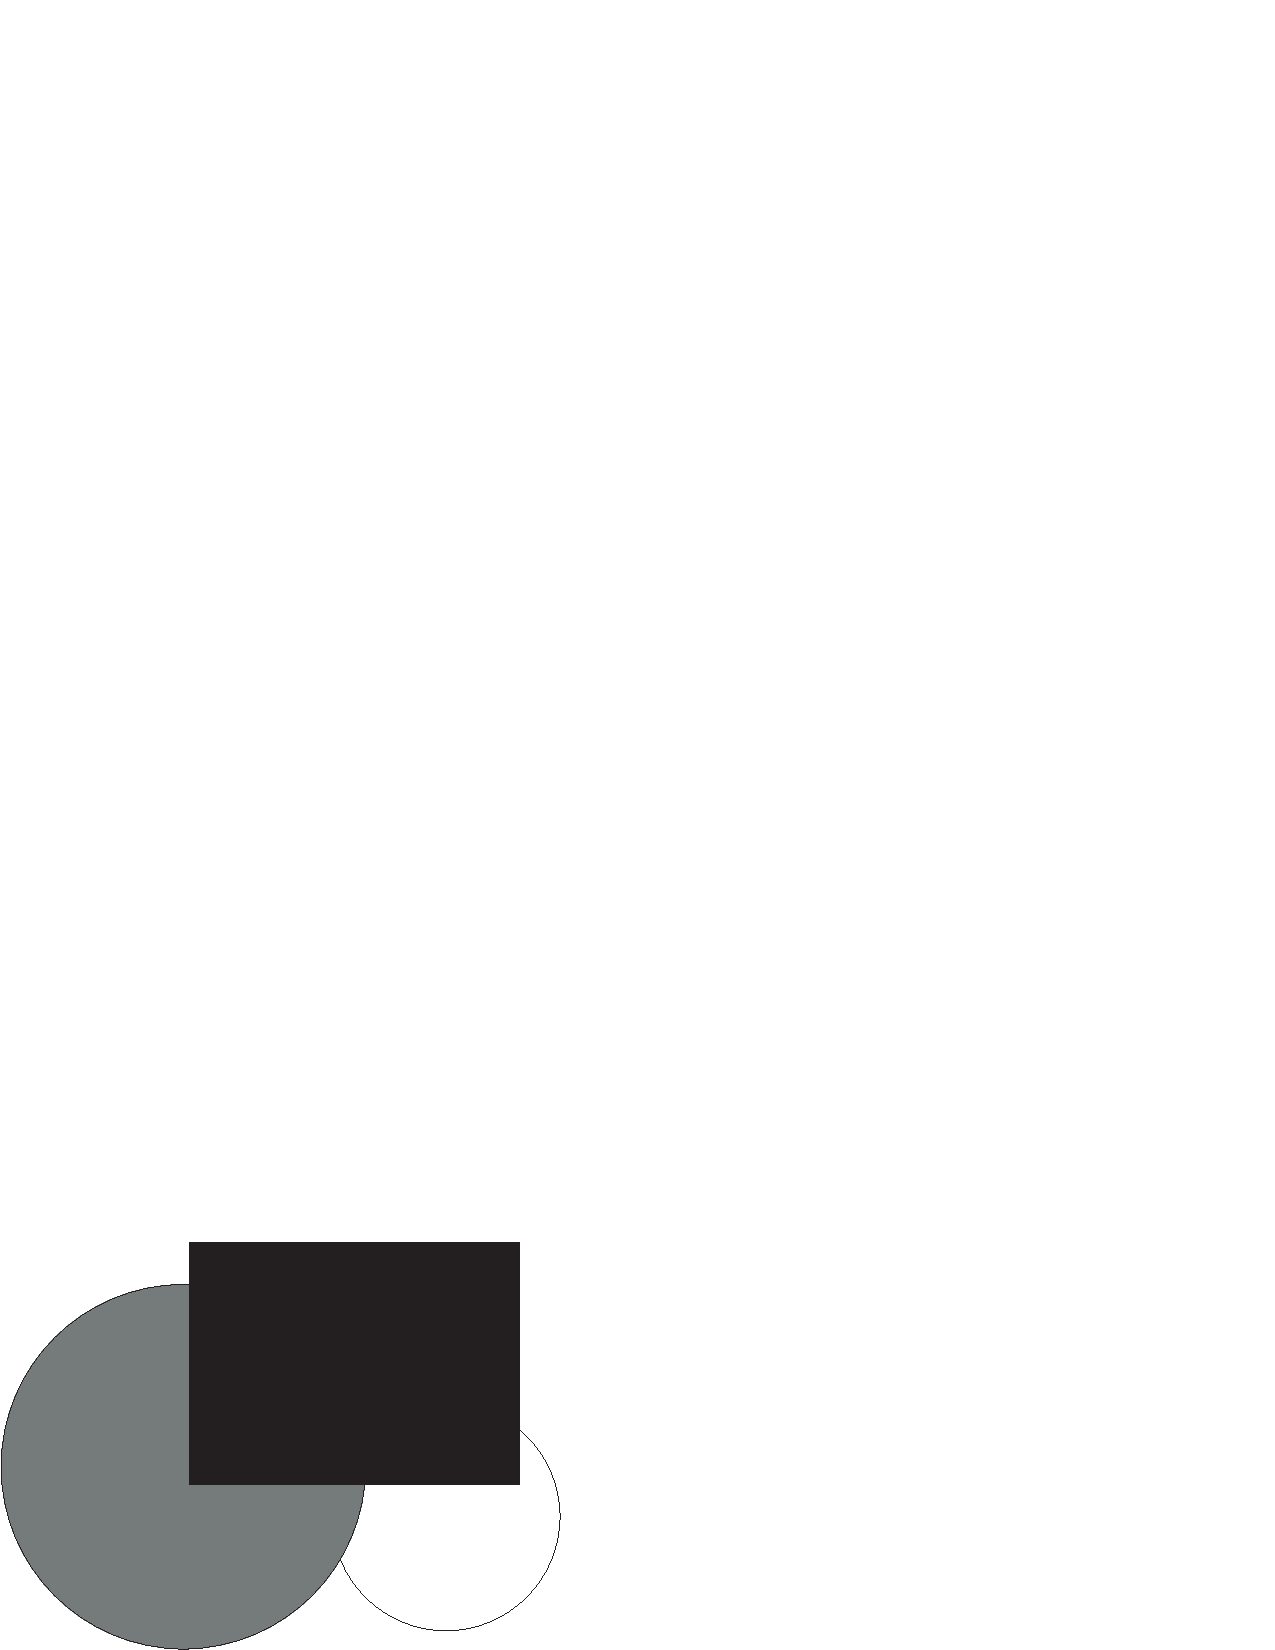
\includegraphics[width=.5\textwidth]{figures/example_fig}
  \caption[An example figure.]{An example figure. If the caption is
    shorter than one line, it is centered. If it goes over more than
    one line, it is left and right justified. Furthermore, it is
    suggested that an alternative short caption is given in order to
    produce a good list of figures.}
  \label{fig:example}
\end{figure}

\begin{table}[tbp]
  \centering
  \begin{tabular}{c|c}
    Age  & IQ  \\ 
    \hline
    10   & 100 \\
    20   & 100 \\
    30   & 150 \\
    40   & 100 \\
    50   & 100
  \end{tabular}
  \caption{An example table.}
  \label{tab:example}
\end{table}

\begin{table}[tbp]
  \centering
  \csvautobooktabular{figures/ageiq.csv}
  \caption{An example table using simplecsv.}
  \label{tab:examplecsv}
\end{table}

The captions are placed \emph{below} both for the figures and the
tables. The caption is set in 9pt. If the caption is shorter than one
line, it is centered.

\subsection{Gnuplot}
There are many ways to include graphs in your document.  Figure~\ref{fig:exgnuplotex} for including a file generated by gnuplot and saved as \texttt{gnuplotgraph1.tex}. 
%Figure~\ref{fig:exgnuplotintegrate} shows how to include the script to generate a graph direction in \LaTeX.

\begin{figure}[htp]  %t top, b bottom, p page | you can also use h to try to get the figure to appear at the current location
  \centering
  % GNUPLOT: LaTeX picture
\setlength{\unitlength}{0.240900pt}
\ifx\plotpoint\undefined\newsavebox{\plotpoint}\fi
\begin{picture}(1500,900)(0,0)
\sbox{\plotpoint}{\rule[-0.200pt]{0.400pt}{0.400pt}}%
\put(130.0,82.0){\rule[-0.200pt]{4.818pt}{0.400pt}}
\put(110,82){\makebox(0,0)[r]{-1}}
\put(1419.0,82.0){\rule[-0.200pt]{4.818pt}{0.400pt}}
\put(130.0,151.0){\rule[-0.200pt]{4.818pt}{0.400pt}}
\put(110,151){\makebox(0,0)[r]{-0.8}}
\put(1419.0,151.0){\rule[-0.200pt]{4.818pt}{0.400pt}}
\put(130.0,221.0){\rule[-0.200pt]{4.818pt}{0.400pt}}
\put(110,221){\makebox(0,0)[r]{-0.6}}
\put(1419.0,221.0){\rule[-0.200pt]{4.818pt}{0.400pt}}
\put(130.0,290.0){\rule[-0.200pt]{4.818pt}{0.400pt}}
\put(110,290){\makebox(0,0)[r]{-0.4}}
\put(1419.0,290.0){\rule[-0.200pt]{4.818pt}{0.400pt}}
\put(130.0,360.0){\rule[-0.200pt]{4.818pt}{0.400pt}}
\put(110,360){\makebox(0,0)[r]{-0.2}}
\put(1419.0,360.0){\rule[-0.200pt]{4.818pt}{0.400pt}}
\put(130.0,429.0){\rule[-0.200pt]{4.818pt}{0.400pt}}
\put(110,429){\makebox(0,0)[r]{ 0}}
\put(1419.0,429.0){\rule[-0.200pt]{4.818pt}{0.400pt}}
\put(130.0,498.0){\rule[-0.200pt]{4.818pt}{0.400pt}}
\put(110,498){\makebox(0,0)[r]{ 0.2}}
\put(1419.0,498.0){\rule[-0.200pt]{4.818pt}{0.400pt}}
\put(130.0,568.0){\rule[-0.200pt]{4.818pt}{0.400pt}}
\put(110,568){\makebox(0,0)[r]{ 0.4}}
\put(1419.0,568.0){\rule[-0.200pt]{4.818pt}{0.400pt}}
\put(130.0,637.0){\rule[-0.200pt]{4.818pt}{0.400pt}}
\put(110,637){\makebox(0,0)[r]{ 0.6}}
\put(1419.0,637.0){\rule[-0.200pt]{4.818pt}{0.400pt}}
\put(130.0,707.0){\rule[-0.200pt]{4.818pt}{0.400pt}}
\put(110,707){\makebox(0,0)[r]{ 0.8}}
\put(1419.0,707.0){\rule[-0.200pt]{4.818pt}{0.400pt}}
\put(130.0,776.0){\rule[-0.200pt]{4.818pt}{0.400pt}}
\put(110,776){\makebox(0,0)[r]{ 1}}
\put(1419.0,776.0){\rule[-0.200pt]{4.818pt}{0.400pt}}
\put(130.0,82.0){\rule[-0.200pt]{0.400pt}{4.818pt}}
\put(130,41){\makebox(0,0){-10}}
\put(130.0,756.0){\rule[-0.200pt]{0.400pt}{4.818pt}}
\put(457.0,82.0){\rule[-0.200pt]{0.400pt}{4.818pt}}
\put(457,41){\makebox(0,0){-5}}
\put(457.0,756.0){\rule[-0.200pt]{0.400pt}{4.818pt}}
\put(785.0,82.0){\rule[-0.200pt]{0.400pt}{4.818pt}}
\put(785,41){\makebox(0,0){ 0}}
\put(785.0,756.0){\rule[-0.200pt]{0.400pt}{4.818pt}}
\put(1112.0,82.0){\rule[-0.200pt]{0.400pt}{4.818pt}}
\put(1112,41){\makebox(0,0){ 5}}
\put(1112.0,756.0){\rule[-0.200pt]{0.400pt}{4.818pt}}
\put(1439.0,82.0){\rule[-0.200pt]{0.400pt}{4.818pt}}
\put(1439,41){\makebox(0,0){ 10}}
\put(1439.0,756.0){\rule[-0.200pt]{0.400pt}{4.818pt}}
\put(130.0,82.0){\rule[-0.200pt]{0.400pt}{167.185pt}}
\put(130.0,82.0){\rule[-0.200pt]{315.338pt}{0.400pt}}
\put(1439.0,82.0){\rule[-0.200pt]{0.400pt}{167.185pt}}
\put(130.0,776.0){\rule[-0.200pt]{315.338pt}{0.400pt}}
\put(784,838){\makebox(0,0){Test of $y=sin(x)$}}
\put(785,429){\makebox(0,0)[l]{$y=sin(x)$}}
\put(1279,736){\makebox(0,0)[r]{sin(x)}}
\put(1299.0,736.0){\rule[-0.200pt]{24.090pt}{0.400pt}}
\put(130,618){\usebox{\plotpoint}}
\multiput(130.58,609.67)(0.493,-2.439){23}{\rule{0.119pt}{2.008pt}}
\multiput(129.17,613.83)(13.000,-57.833){2}{\rule{0.400pt}{1.004pt}}
\multiput(143.58,546.90)(0.493,-2.677){23}{\rule{0.119pt}{2.192pt}}
\multiput(142.17,551.45)(13.000,-63.450){2}{\rule{0.400pt}{1.096pt}}
\multiput(156.58,479.28)(0.494,-2.553){25}{\rule{0.119pt}{2.100pt}}
\multiput(155.17,483.64)(14.000,-65.641){2}{\rule{0.400pt}{1.050pt}}
\multiput(170.58,408.77)(0.493,-2.717){23}{\rule{0.119pt}{2.223pt}}
\multiput(169.17,413.39)(13.000,-64.386){2}{\rule{0.400pt}{1.112pt}}
\multiput(183.58,340.15)(0.493,-2.598){23}{\rule{0.119pt}{2.131pt}}
\multiput(182.17,344.58)(13.000,-61.577){2}{\rule{0.400pt}{1.065pt}}
\multiput(196.58,274.92)(0.493,-2.360){23}{\rule{0.119pt}{1.946pt}}
\multiput(195.17,278.96)(13.000,-55.961){2}{\rule{0.400pt}{0.973pt}}
\multiput(209.58,216.42)(0.494,-1.892){25}{\rule{0.119pt}{1.586pt}}
\multiput(208.17,219.71)(14.000,-48.709){2}{\rule{0.400pt}{0.793pt}}
\multiput(223.58,165.35)(0.493,-1.607){23}{\rule{0.119pt}{1.362pt}}
\multiput(222.17,168.17)(13.000,-38.174){2}{\rule{0.400pt}{0.681pt}}
\multiput(236.58,125.75)(0.493,-1.171){23}{\rule{0.119pt}{1.023pt}}
\multiput(235.17,127.88)(13.000,-27.877){2}{\rule{0.400pt}{0.512pt}}
\multiput(249.58,97.67)(0.493,-0.576){23}{\rule{0.119pt}{0.562pt}}
\multiput(248.17,98.83)(13.000,-13.834){2}{\rule{0.400pt}{0.281pt}}
\put(262,83.17){\rule{2.700pt}{0.400pt}}
\multiput(262.00,84.17)(7.396,-2.000){2}{\rule{1.350pt}{0.400pt}}
\multiput(275.00,83.58)(0.582,0.492){21}{\rule{0.567pt}{0.119pt}}
\multiput(275.00,82.17)(12.824,12.000){2}{\rule{0.283pt}{0.400pt}}
\multiput(289.58,95.00)(0.493,1.012){23}{\rule{0.119pt}{0.900pt}}
\multiput(288.17,95.00)(13.000,24.132){2}{\rule{0.400pt}{0.450pt}}
\multiput(302.58,121.00)(0.493,1.527){23}{\rule{0.119pt}{1.300pt}}
\multiput(301.17,121.00)(13.000,36.302){2}{\rule{0.400pt}{0.650pt}}
\multiput(315.58,160.00)(0.493,1.924){23}{\rule{0.119pt}{1.608pt}}
\multiput(314.17,160.00)(13.000,45.663){2}{\rule{0.400pt}{0.804pt}}
\multiput(328.58,209.00)(0.494,2.113){25}{\rule{0.119pt}{1.757pt}}
\multiput(327.17,209.00)(14.000,54.353){2}{\rule{0.400pt}{0.879pt}}
\multiput(342.58,267.00)(0.493,2.558){23}{\rule{0.119pt}{2.100pt}}
\multiput(341.17,267.00)(13.000,60.641){2}{\rule{0.400pt}{1.050pt}}
\multiput(355.58,332.00)(0.493,2.717){23}{\rule{0.119pt}{2.223pt}}
\multiput(354.17,332.00)(13.000,64.386){2}{\rule{0.400pt}{1.112pt}}
\multiput(368.58,401.00)(0.493,2.757){23}{\rule{0.119pt}{2.254pt}}
\multiput(367.17,401.00)(13.000,65.322){2}{\rule{0.400pt}{1.127pt}}
\multiput(381.58,471.00)(0.493,2.677){23}{\rule{0.119pt}{2.192pt}}
\multiput(380.17,471.00)(13.000,63.450){2}{\rule{0.400pt}{1.096pt}}
\multiput(394.58,539.00)(0.494,2.333){25}{\rule{0.119pt}{1.929pt}}
\multiput(393.17,539.00)(14.000,59.997){2}{\rule{0.400pt}{0.964pt}}
\multiput(408.58,603.00)(0.493,2.241){23}{\rule{0.119pt}{1.854pt}}
\multiput(407.17,603.00)(13.000,53.152){2}{\rule{0.400pt}{0.927pt}}
\multiput(421.58,660.00)(0.493,1.845){23}{\rule{0.119pt}{1.546pt}}
\multiput(420.17,660.00)(13.000,43.791){2}{\rule{0.400pt}{0.773pt}}
\multiput(434.58,707.00)(0.493,1.408){23}{\rule{0.119pt}{1.208pt}}
\multiput(433.17,707.00)(13.000,33.493){2}{\rule{0.400pt}{0.604pt}}
\multiput(447.58,743.00)(0.494,0.827){25}{\rule{0.119pt}{0.757pt}}
\multiput(446.17,743.00)(14.000,21.429){2}{\rule{0.400pt}{0.379pt}}
\multiput(461.00,766.58)(0.652,0.491){17}{\rule{0.620pt}{0.118pt}}
\multiput(461.00,765.17)(11.713,10.000){2}{\rule{0.310pt}{0.400pt}}
\multiput(474.00,774.93)(1.378,-0.477){7}{\rule{1.140pt}{0.115pt}}
\multiput(474.00,775.17)(10.634,-5.000){2}{\rule{0.570pt}{0.400pt}}
\multiput(487.58,768.29)(0.493,-0.695){23}{\rule{0.119pt}{0.654pt}}
\multiput(486.17,769.64)(13.000,-16.643){2}{\rule{0.400pt}{0.327pt}}
\multiput(500.58,748.50)(0.493,-1.250){23}{\rule{0.119pt}{1.085pt}}
\multiput(499.17,750.75)(13.000,-29.749){2}{\rule{0.400pt}{0.542pt}}
\multiput(513.58,715.37)(0.494,-1.599){25}{\rule{0.119pt}{1.357pt}}
\multiput(512.17,718.18)(14.000,-41.183){2}{\rule{0.400pt}{0.679pt}}
\multiput(527.58,669.82)(0.493,-2.083){23}{\rule{0.119pt}{1.731pt}}
\multiput(526.17,673.41)(13.000,-49.408){2}{\rule{0.400pt}{0.865pt}}
\multiput(540.58,615.67)(0.493,-2.439){23}{\rule{0.119pt}{2.008pt}}
\multiput(539.17,619.83)(13.000,-57.833){2}{\rule{0.400pt}{1.004pt}}
\multiput(553.58,553.03)(0.493,-2.638){23}{\rule{0.119pt}{2.162pt}}
\multiput(552.17,557.51)(13.000,-62.514){2}{\rule{0.400pt}{1.081pt}}
\multiput(566.58,486.28)(0.494,-2.553){25}{\rule{0.119pt}{2.100pt}}
\multiput(565.17,490.64)(14.000,-65.641){2}{\rule{0.400pt}{1.050pt}}
\multiput(580.58,415.77)(0.493,-2.717){23}{\rule{0.119pt}{2.223pt}}
\multiput(579.17,420.39)(13.000,-64.386){2}{\rule{0.400pt}{1.112pt}}
\multiput(593.58,347.03)(0.493,-2.638){23}{\rule{0.119pt}{2.162pt}}
\multiput(592.17,351.51)(13.000,-62.514){2}{\rule{0.400pt}{1.081pt}}
\multiput(606.58,280.79)(0.493,-2.400){23}{\rule{0.119pt}{1.977pt}}
\multiput(605.17,284.90)(13.000,-56.897){2}{\rule{0.400pt}{0.988pt}}
\multiput(619.58,220.94)(0.493,-2.043){23}{\rule{0.119pt}{1.700pt}}
\multiput(618.17,224.47)(13.000,-48.472){2}{\rule{0.400pt}{0.850pt}}
\multiput(632.58,170.48)(0.494,-1.562){25}{\rule{0.119pt}{1.329pt}}
\multiput(631.17,173.24)(14.000,-40.242){2}{\rule{0.400pt}{0.664pt}}
\multiput(646.58,128.75)(0.493,-1.171){23}{\rule{0.119pt}{1.023pt}}
\multiput(645.17,130.88)(13.000,-27.877){2}{\rule{0.400pt}{0.512pt}}
\multiput(659.58,100.41)(0.493,-0.655){23}{\rule{0.119pt}{0.623pt}}
\multiput(658.17,101.71)(13.000,-15.707){2}{\rule{0.400pt}{0.312pt}}
\multiput(672.00,84.95)(2.695,-0.447){3}{\rule{1.833pt}{0.108pt}}
\multiput(672.00,85.17)(9.195,-3.000){2}{\rule{0.917pt}{0.400pt}}
\multiput(685.00,83.58)(0.704,0.491){17}{\rule{0.660pt}{0.118pt}}
\multiput(685.00,82.17)(12.630,10.000){2}{\rule{0.330pt}{0.400pt}}
\multiput(699.58,93.00)(0.493,0.972){23}{\rule{0.119pt}{0.869pt}}
\multiput(698.17,93.00)(13.000,23.196){2}{\rule{0.400pt}{0.435pt}}
\multiput(712.58,118.00)(0.493,1.448){23}{\rule{0.119pt}{1.238pt}}
\multiput(711.17,118.00)(13.000,34.430){2}{\rule{0.400pt}{0.619pt}}
\multiput(725.58,155.00)(0.493,1.924){23}{\rule{0.119pt}{1.608pt}}
\multiput(724.17,155.00)(13.000,45.663){2}{\rule{0.400pt}{0.804pt}}
\multiput(738.58,204.00)(0.493,2.241){23}{\rule{0.119pt}{1.854pt}}
\multiput(737.17,204.00)(13.000,53.152){2}{\rule{0.400pt}{0.927pt}}
\multiput(751.58,261.00)(0.494,2.333){25}{\rule{0.119pt}{1.929pt}}
\multiput(750.17,261.00)(14.000,59.997){2}{\rule{0.400pt}{0.964pt}}
\multiput(765.58,325.00)(0.493,2.717){23}{\rule{0.119pt}{2.223pt}}
\multiput(764.17,325.00)(13.000,64.386){2}{\rule{0.400pt}{1.112pt}}
\multiput(778.58,394.00)(0.493,2.757){23}{\rule{0.119pt}{2.254pt}}
\multiput(777.17,394.00)(13.000,65.322){2}{\rule{0.400pt}{1.127pt}}
\multiput(791.58,464.00)(0.493,2.717){23}{\rule{0.119pt}{2.223pt}}
\multiput(790.17,464.00)(13.000,64.386){2}{\rule{0.400pt}{1.112pt}}
\multiput(804.58,533.00)(0.494,2.333){25}{\rule{0.119pt}{1.929pt}}
\multiput(803.17,533.00)(14.000,59.997){2}{\rule{0.400pt}{0.964pt}}
\multiput(818.58,597.00)(0.493,2.241){23}{\rule{0.119pt}{1.854pt}}
\multiput(817.17,597.00)(13.000,53.152){2}{\rule{0.400pt}{0.927pt}}
\multiput(831.58,654.00)(0.493,1.924){23}{\rule{0.119pt}{1.608pt}}
\multiput(830.17,654.00)(13.000,45.663){2}{\rule{0.400pt}{0.804pt}}
\multiput(844.58,703.00)(0.493,1.448){23}{\rule{0.119pt}{1.238pt}}
\multiput(843.17,703.00)(13.000,34.430){2}{\rule{0.400pt}{0.619pt}}
\multiput(857.58,740.00)(0.493,0.972){23}{\rule{0.119pt}{0.869pt}}
\multiput(856.17,740.00)(13.000,23.196){2}{\rule{0.400pt}{0.435pt}}
\multiput(870.00,765.58)(0.704,0.491){17}{\rule{0.660pt}{0.118pt}}
\multiput(870.00,764.17)(12.630,10.000){2}{\rule{0.330pt}{0.400pt}}
\multiput(884.00,773.95)(2.695,-0.447){3}{\rule{1.833pt}{0.108pt}}
\multiput(884.00,774.17)(9.195,-3.000){2}{\rule{0.917pt}{0.400pt}}
\multiput(897.58,769.41)(0.493,-0.655){23}{\rule{0.119pt}{0.623pt}}
\multiput(896.17,770.71)(13.000,-15.707){2}{\rule{0.400pt}{0.312pt}}
\multiput(910.58,750.75)(0.493,-1.171){23}{\rule{0.119pt}{1.023pt}}
\multiput(909.17,752.88)(13.000,-27.877){2}{\rule{0.400pt}{0.512pt}}
\multiput(923.58,719.48)(0.494,-1.562){25}{\rule{0.119pt}{1.329pt}}
\multiput(922.17,722.24)(14.000,-40.242){2}{\rule{0.400pt}{0.664pt}}
\multiput(937.58,674.94)(0.493,-2.043){23}{\rule{0.119pt}{1.700pt}}
\multiput(936.17,678.47)(13.000,-48.472){2}{\rule{0.400pt}{0.850pt}}
\multiput(950.58,621.79)(0.493,-2.400){23}{\rule{0.119pt}{1.977pt}}
\multiput(949.17,625.90)(13.000,-56.897){2}{\rule{0.400pt}{0.988pt}}
\multiput(963.58,560.03)(0.493,-2.638){23}{\rule{0.119pt}{2.162pt}}
\multiput(962.17,564.51)(13.000,-62.514){2}{\rule{0.400pt}{1.081pt}}
\multiput(976.58,492.77)(0.493,-2.717){23}{\rule{0.119pt}{2.223pt}}
\multiput(975.17,497.39)(13.000,-64.386){2}{\rule{0.400pt}{1.112pt}}
\multiput(989.58,424.28)(0.494,-2.553){25}{\rule{0.119pt}{2.100pt}}
\multiput(988.17,428.64)(14.000,-65.641){2}{\rule{0.400pt}{1.050pt}}
\multiput(1003.58,354.03)(0.493,-2.638){23}{\rule{0.119pt}{2.162pt}}
\multiput(1002.17,358.51)(13.000,-62.514){2}{\rule{0.400pt}{1.081pt}}
\multiput(1016.58,287.67)(0.493,-2.439){23}{\rule{0.119pt}{2.008pt}}
\multiput(1015.17,291.83)(13.000,-57.833){2}{\rule{0.400pt}{1.004pt}}
\multiput(1029.58,226.82)(0.493,-2.083){23}{\rule{0.119pt}{1.731pt}}
\multiput(1028.17,230.41)(13.000,-49.408){2}{\rule{0.400pt}{0.865pt}}
\multiput(1042.58,175.37)(0.494,-1.599){25}{\rule{0.119pt}{1.357pt}}
\multiput(1041.17,178.18)(14.000,-41.183){2}{\rule{0.400pt}{0.679pt}}
\multiput(1056.58,132.50)(0.493,-1.250){23}{\rule{0.119pt}{1.085pt}}
\multiput(1055.17,134.75)(13.000,-29.749){2}{\rule{0.400pt}{0.542pt}}
\multiput(1069.58,102.29)(0.493,-0.695){23}{\rule{0.119pt}{0.654pt}}
\multiput(1068.17,103.64)(13.000,-16.643){2}{\rule{0.400pt}{0.327pt}}
\multiput(1082.00,85.93)(1.378,-0.477){7}{\rule{1.140pt}{0.115pt}}
\multiput(1082.00,86.17)(10.634,-5.000){2}{\rule{0.570pt}{0.400pt}}
\multiput(1095.00,82.58)(0.652,0.491){17}{\rule{0.620pt}{0.118pt}}
\multiput(1095.00,81.17)(11.713,10.000){2}{\rule{0.310pt}{0.400pt}}
\multiput(1108.58,92.00)(0.494,0.827){25}{\rule{0.119pt}{0.757pt}}
\multiput(1107.17,92.00)(14.000,21.429){2}{\rule{0.400pt}{0.379pt}}
\multiput(1122.58,115.00)(0.493,1.408){23}{\rule{0.119pt}{1.208pt}}
\multiput(1121.17,115.00)(13.000,33.493){2}{\rule{0.400pt}{0.604pt}}
\multiput(1135.58,151.00)(0.493,1.845){23}{\rule{0.119pt}{1.546pt}}
\multiput(1134.17,151.00)(13.000,43.791){2}{\rule{0.400pt}{0.773pt}}
\multiput(1148.58,198.00)(0.493,2.241){23}{\rule{0.119pt}{1.854pt}}
\multiput(1147.17,198.00)(13.000,53.152){2}{\rule{0.400pt}{0.927pt}}
\multiput(1161.58,255.00)(0.494,2.333){25}{\rule{0.119pt}{1.929pt}}
\multiput(1160.17,255.00)(14.000,59.997){2}{\rule{0.400pt}{0.964pt}}
\multiput(1175.58,319.00)(0.493,2.677){23}{\rule{0.119pt}{2.192pt}}
\multiput(1174.17,319.00)(13.000,63.450){2}{\rule{0.400pt}{1.096pt}}
\multiput(1188.58,387.00)(0.493,2.757){23}{\rule{0.119pt}{2.254pt}}
\multiput(1187.17,387.00)(13.000,65.322){2}{\rule{0.400pt}{1.127pt}}
\multiput(1201.58,457.00)(0.493,2.717){23}{\rule{0.119pt}{2.223pt}}
\multiput(1200.17,457.00)(13.000,64.386){2}{\rule{0.400pt}{1.112pt}}
\multiput(1214.58,526.00)(0.493,2.558){23}{\rule{0.119pt}{2.100pt}}
\multiput(1213.17,526.00)(13.000,60.641){2}{\rule{0.400pt}{1.050pt}}
\multiput(1227.58,591.00)(0.494,2.113){25}{\rule{0.119pt}{1.757pt}}
\multiput(1226.17,591.00)(14.000,54.353){2}{\rule{0.400pt}{0.879pt}}
\multiput(1241.58,649.00)(0.493,1.924){23}{\rule{0.119pt}{1.608pt}}
\multiput(1240.17,649.00)(13.000,45.663){2}{\rule{0.400pt}{0.804pt}}
\multiput(1254.58,698.00)(0.493,1.527){23}{\rule{0.119pt}{1.300pt}}
\multiput(1253.17,698.00)(13.000,36.302){2}{\rule{0.400pt}{0.650pt}}
\multiput(1267.58,737.00)(0.493,1.012){23}{\rule{0.119pt}{0.900pt}}
\multiput(1266.17,737.00)(13.000,24.132){2}{\rule{0.400pt}{0.450pt}}
\multiput(1280.00,763.58)(0.582,0.492){21}{\rule{0.567pt}{0.119pt}}
\multiput(1280.00,762.17)(12.824,12.000){2}{\rule{0.283pt}{0.400pt}}
\put(1294,773.17){\rule{2.700pt}{0.400pt}}
\multiput(1294.00,774.17)(7.396,-2.000){2}{\rule{1.350pt}{0.400pt}}
\multiput(1307.58,770.67)(0.493,-0.576){23}{\rule{0.119pt}{0.562pt}}
\multiput(1306.17,771.83)(13.000,-13.834){2}{\rule{0.400pt}{0.281pt}}
\multiput(1320.58,753.75)(0.493,-1.171){23}{\rule{0.119pt}{1.023pt}}
\multiput(1319.17,755.88)(13.000,-27.877){2}{\rule{0.400pt}{0.512pt}}
\multiput(1333.58,722.35)(0.493,-1.607){23}{\rule{0.119pt}{1.362pt}}
\multiput(1332.17,725.17)(13.000,-38.174){2}{\rule{0.400pt}{0.681pt}}
\multiput(1346.58,680.42)(0.494,-1.892){25}{\rule{0.119pt}{1.586pt}}
\multiput(1345.17,683.71)(14.000,-48.709){2}{\rule{0.400pt}{0.793pt}}
\multiput(1360.58,626.92)(0.493,-2.360){23}{\rule{0.119pt}{1.946pt}}
\multiput(1359.17,630.96)(13.000,-55.961){2}{\rule{0.400pt}{0.973pt}}
\multiput(1373.58,566.15)(0.493,-2.598){23}{\rule{0.119pt}{2.131pt}}
\multiput(1372.17,570.58)(13.000,-61.577){2}{\rule{0.400pt}{1.065pt}}
\multiput(1386.58,499.77)(0.493,-2.717){23}{\rule{0.119pt}{2.223pt}}
\multiput(1385.17,504.39)(13.000,-64.386){2}{\rule{0.400pt}{1.112pt}}
\multiput(1399.58,431.28)(0.494,-2.553){25}{\rule{0.119pt}{2.100pt}}
\multiput(1398.17,435.64)(14.000,-65.641){2}{\rule{0.400pt}{1.050pt}}
\multiput(1413.58,360.90)(0.493,-2.677){23}{\rule{0.119pt}{2.192pt}}
\multiput(1412.17,365.45)(13.000,-63.450){2}{\rule{0.400pt}{1.096pt}}
\multiput(1426.58,293.67)(0.493,-2.439){23}{\rule{0.119pt}{2.008pt}}
\multiput(1425.17,297.83)(13.000,-57.833){2}{\rule{0.400pt}{1.004pt}}
\put(130.0,82.0){\rule[-0.200pt]{0.400pt}{167.185pt}}
\put(130.0,82.0){\rule[-0.200pt]{315.338pt}{0.400pt}}
\put(1439.0,82.0){\rule[-0.200pt]{0.400pt}{167.185pt}}
\put(130.0,776.0){\rule[-0.200pt]{315.338pt}{0.400pt}}
\end{picture}

  \caption[An example graph.]{This is a gnuplot graph of $y=\sin(x)$. Notice how the \LaTeX{} fonts are preserved in the graph. This is done using gnuplot and the simple text file included in the sample template.}
  \label{fig:exgnuplotex}
\end{figure}

\begin{figure}[htp]  %t top, b bottom, p page | you can also use h to try to get the figure to appear at the current location
  \centering
    \begin{gnuplot}[terminal=epslatex, terminaloptions=color]
        set xlabel "Age" 
        set ylabel "IQ" 
        set key autotitle columnhead
        set title "Age vs Average IQ"
        set yrange [0:160]
        set datafile separator ","
        plot "figures/ageiq.csv" using 1:2 with boxes 
    \end{gnuplot}
  \caption[An example of Integrated Graph]{This is a gnuplot graph read from a file}
  \label{fig:exgnuplotintegratefile}
\end{figure}


%\begin{figure}[htp]  %t top, b bottom, p page | you can also use h to try to get the figure to appear at the urrent location
%  \centering
%    \begin{gnuplot}[terminal=pdf, terminaloptions=color]
%        unset hidden3d
%        set view 102,57,1
%        set xtics offset -1.3,-0.3
%        set ytics offset 0,-0.5
%        set samples 21
%        set isosample 11
%        set xlabel "Confidence" offset -3,-2
%        set ylabel "Resilience" offset 3,-2
%        set zlabel "Rate of change" offset 2, 6
%        set title "Rate of feat change in relation to Resilience and Confidence"
%        set xrange [0:1]
%        set yrange [0:1]
%        splot 1-((1-x)*y)
%    \end{gnuplot}
%  \caption[An example 3D graph.]{This is a gnuplot graph of $1-((1-x)*y)$. This is code that is compiles during the \LaTeX{} processing. This is done using gnuplottex, it could also come from a file}
%  \label{fig:exgnuplotintegrate}
%\end{figure}

\section{Quotes}
\label{sec:Quotes} % this allows you to refer to this section number using \ref{sec:Quotes}

Quotes are inserted using the standard \LaTeX\ \texttt{quote}
environment. The environment has been changed so that a 9pt font is
used:

\begin{quote}
  ``And I looked, and, behold, a whirlwind came out of the north, a
  great cloud, and a fire infolding itself, and a brightness was about
  it, and out of the midst thereof as the colour of amber, out of the
  midst of the fire. Also out of the midst thereof came the likeness
  of four living creatures.''
\end{quote}

\section{Lists}
\label{sec:lists}

Point lists and enumerated lists are made by using the standard
\texttt{itemize} and \texttt{enumerate} environments, respectively.
The spacing is going to be changed in accordance with the specification. For
\texttt{itemize}, the results look like this:
\begin{itemize}
	\item First item.
	\item Second item. Here I will put some long text, just to illustrate.
	  Here I will put some long text, just to illustrate. Here I will put
	  some long text, just to illustrate. Here I will put some long text,
	  just to illustrate.
	\item Third item also has subitems:
	  \begin{itemize}
		  \item First subitem.
		  \item Second subitem.
		  \item Third subitem.
	  \end{itemize}
\end{itemize}
and for \texttt{enumerate} like this:
\begin{enumerate}
	\item First item.
	\item Second item. Here I will put some long text, just to illustrate.
	  Here I will put some long text, just to illustrate. Here I will put
	  some long text, just to illustrate. Here I will put some long text,
	  just to illustrate.
	\item Third item also has subitems:
	  \begin{enumerate}
		  \item First subitem.
		  \item Second subitem.
		  \item Third subitem.
	  \end{enumerate}
\end{enumerate}

You may also want to use descriptive lists
\begin{description}
	\item[First] the first item.
	\item[Second] the second item. Here I will put some long text, just to illustrate.
	  Here I will put some long text, just to illustrate. Here I will put
	  some long text, just to illustrate. Here I will put some long text,
	  just to illustrate.
	\item [What now] the third item also has subitems:
	  \begin{enumerate}
		  \item First subitem.
		  \item Second subitem.
		  \item Third subitem.
	  \end{enumerate}
\end{description}


\section{Bibliographic References}

There are two distinct styles of referencing which can be used within the Masters thesis, Vancouver for Computer Science and Harvard for Interaction Design.

In Computer Science we generally use the Vancouver style with numbered references.  
I have added a boolean option \verb|\setboolean{HarvardCitations}{false}|  Havard style if false for computer science and true for interaction design.
 


For Harvard style referencing, you use the \texttt{citep} and \texttt{citet} style of citation. 
These give parentheses around the citation or the name of the author as text with the year in parentheses.  
If you want the citation to be read in a sentence then you use  \texttt{citet}. 
If you want it to be just parenthetical to the sentence at the end, then use \texttt{citep}.

\section{Code}

For code listing (see Figure~\ref{fig:HelloWorldC++} and Figure~\ref{fig:PythonCode}) we have included the listings package so that you can easily include formatted code.  It does not have code highlighting but it retains the structure of the code.  For more documentation on listings on wikibooks \footnote{\url{https://en.wikibooks.org/wiki/LaTeX/Source_Code_Listings}}


\begin{figure}[tp] 
  \centering
\lstset{language=C++,
        morecomment=[l][\color{darkgreen}]{\#}}
\begin{lstlisting}
    #include<stdio.h>
    #include<iostream>
    // A comment
    int main(void)
    {
    printf("Hello World\n");
    return 0;
    }
\end{lstlisting}
  \caption[Hello World C++]{The code listing for Hello World in C++, with colour syntax highlighting.}
  \label{fig:HelloWorldC++}
\end{figure}

You could also use Python code listings by changing the language of the code block

\begin{figure}[tp] 
  \centering
\lstset{language=Python}
\begin{lstlisting}
import numpy as np
x = 1
a = np.array([[1.0, 2.0], [3.0, 4.0]])
if x == 1:
    # indented four spaces
    print("x is 1.")
    print("Hello World")
    print(a)
\end{lstlisting}
  \caption[Python code example]{The code listing for a Python increment a matrix example}
  \label{fig:PythonCode}
\end{figure}

\section{Statistical Analysis}

Many of you will need to use statistics to reject null hypotheses.  There are many statistical packages and ways of analysing data.  Your supervisor should be able to direct you to the type of analytically tool that will allow you to make justifiable claims.

There are some key things to remember.  If you want to make a claim that thing A is better than thing B, then you are rejecting the null hypothesis that they are the same. Equation~\ref{H0mean} states the null hypothesis as the mean of sample 1 ($\mu_1$) is the same as the mean of sample 2 ($\mu_2$). For example if you were measuring height of men and women you would state that the null hypothesis is that men and women are the same height, then you measure 100 men and 100 women and calculate the mean and standard variation of their height. 
\begin{equation} 
\label{H0mean}
    H_0 : \mu_1 = \mu_2
\end{equation}

The t-test can be used to see what the probability $p$ of seeing the values in the sample that you coming from the same actual population. If you have a $p<0.05$ you have a 95\% probability that the samples are actually different.

Thus you set up the evaluation and show that there is a very low probability that the difference you see is caused by sampling error and therefor they are not the same.  The t-test does this for normally distributed scalar values of data. If you are using a Likert Scale then you do not have scalar data, and it may not be normally distributed.

For non-parametric data you need to make a statement about the sampled values~\cite{Kaptein2010}
\begin{equation} 
\label{H0sample}
    H_0 : \phi_1(x) = \phi_2(x)
\end{equation}

There are lots of good sources for understanding statistics for research.  Most of the wikipedia pages are a good entry to the area. For Likert scale analysis there are new tools~\cite{Kaptein2010} which allow for better assessment of the sample sizes we have in most of our Masters thesis projects.

You should also think about learning R the statisical package for doing analysis.  You can download it by searching for "R on windows" or using the link to a windows implementation of R\footnote{\url{https://cran.r-project.org/bin/windows/base/}}


 % could be results
\chapter{Implementation}
\label{chap:implementation}
This has the description of how you actually went about implementing the project.  This should be focused on the interesting challenges and how those related to the project.

There is often the need to layout tables that are long.  We suggest using the sidewaystable mode for this.  You will need to manage the total width of the table to make it fit, but you can see how to do that in the example in Table~\ref{tbl:CBM-MC}.

Writing your own \LaTeX{} tables is very slow, and error prone. There are many converstion tools to help create tables.  The one we used for the sideways table, Table~\ref{tbl:CBM-MC} is LatexKit\footnote{Google plugin for LatexKit \url{https://chrome.google.com/webstore/detail/latexkit/piadpbgaacpbaicjilhfebbfgofomiic}}



% you can also set widths using a new command 
%\newcommand{\Colwidth}{0.08\textwidth}
%\begin{tabular}{l|p{\Colwidth}|p{\Colwidth}|p{\Colwidth}|p{\Colwidth}|p{\Colwidth}|p{\Colwidth}|p{\Colwidth}|p{\Colwidth}|}

\begin{sidewaystable}
\small{
\begin{tabular}{l|cccccccccccccccccc}
Candidate & 1 & 2 & 3 & 4 & 5 & 6 & 7 & 8 & 9 & 10 & 11 & 12 & 13 & 14 & 15 & Num & CBM & Diff. \\
\hline
10001 & 0 & -0.5 & 1 & -0.5 & 1 & -0.5 & -0.5 & 2 & 2 & -2 & 2 & 1.5 & -0.5 & 2 & 2 & 8 & 9 & 0.5 \\
10002 & 0 & 2 & 0 & 0 & 0 & 2 & 2 & 2 & 1 & 1 & 1 & 2 & 0 & 2 & 2 & 10 & 17 & 4.5 \\
10003 & 0 & 2 & -0.5 & 0 & 0 & 2 & 1.5 & 1.5 & 2 & -0.5 & 2 & 1 & 0 & 1.5 & 1.5 & 9 & 14 & 3.5 \\
10004 & 2 & -0.5 & 1 & 0 & 0 & 0 & 2 & 2 & 1 & 0 & 0 & 1 & -0.5 & 1 & -0.5 & 7 & 8.5 & 1.5 \\
10005 & 1 & 0 & 0 & 0 & 0 & 1 & 1 & 0 & 1 & 1 & 1 & 1 & 0 & 1 & 1 & 9 & 9 & -1.5 \\
10006 & 2 & -2 & 0 & -0.5 & 1.5 & 1 & 0 & 2 & 2 & 0 & 2 & 2 & -0.5 & 2 & 2 & 9 & 13.5 & 3 \\
10007 & 1 & -2 & 0 & 0 & 1 & 0 & 1.5 & 2 & 2 & -2 & 0 & 1.5 & -2 & 2 & 1 & 8 & 6 & -2.5 \\
10008 & 2 & 2 & -2 & 0 & 2 & 0 & 2 & 2 & 1.5 & 1.5 & 2 & 1.5 & -0.5 & 2 & 2 & 11 & 18 & 3.5 \\
10009 & 2 & -0.5 & 1 & 0 & -0.5 & 2 & -0.5 & 2 & 2 & 0 & 2 & 2 & -0.5 & -0.5 & 2 & 8 & 12.5 & 4 \\
10010 & 2 & -2 & 2 & 0 & -2 & 2 & 2 & 2 & 1.5 & 1.5 & 1.5 & 2 & 0 & 2 & 2 & 11 & 16.5 & 2 \\
10011 & 2 & 2 & 0 & 1 & 2 & 2 & 2 & -0.5 & 2 & 0 & 2 & 2 & -0.5 & 2 & 2 & 11 & 20 & 5.5 \\
10012 & 2 & 1 & 0 & 2 & -2 & 2 & 2 & 2 & 2 & 0 & 1 & 2 & 0 & 2 & 2 & 11 & 18 & 3.5 \\
10013 & 2 & 2 & 1.5 & 0 & 0 & 2 & 2 & 2 & 1 & 0 & 1 & 2 & -0.5 & 2 & 2 & 11 & 19 & 4.5 \\
10014 & 2 & 2 & 1 & -0.5 & -2 & -2 & 1.5 & 2 & 2 & 1.5 & 2 & 2 & 2 & -0.5 & 2 & 11 & 15 & 0.5 \\
10015 & 1.5 & -2 & 1.5 & 1.5 & 2 & 0 & 2 & 2 & 1.5 & 1 & 2 & -0.5 & 1 & 0 & 1.5 & 11 & 15 & 0.5 \\
10016 & 1 & 2 & 0 & 0 & 1.5 & 0 & 0 & 2 & 1 & 0 & 1 & 1.5 & -0.5 & 1 & 2 & 9 & 12.5 & 2 \\
10018 & 2 & 2 & 1 & 0 & -2 & 0 & -2 & 1.5 & 2 & 1 & 0 & 1.5 & 0 & 1 & 2 & 9 & 10 & -0.5 \\
10019 & 2 & 2 & -2 & 0 & 1.5 & 2 & -0.5 & -0.5 & 1.5 & 1 & 2 & 2 & 0 & 1 & 2 & 10 & 14 & 1.5 \\
10020 & 2 & 2 & 0 & 0 & 2 & 2 & 2 & 2 & -0.5 & 1 & 2 & 2 & 2 & 2 & 2 & 12 & 22.5 & 4.5 \\
\end{tabular}
}
\caption[Confidence Based Marking]{Multichoice marking example data with 15 questions, Number correct (Num), the Confidence Based Marking (CBM) grade,  and the differentiation of knowledge quality (Diff)}
\label{tbl:CBM-MC}

\end{sidewaystable}

%\begin{sidewaystable}
%\centering
%  \csvautobooktabular{figures/largeTable.csv}
%\caption[Autogenerated on Sideways page]{using CSV tables to autogenerate the table in a sideways table. This is not an appropriate use of a sideways table as it is small}
%\label{tbl:dataSetsideways}
%\end{sidewaystable}



\todo{add more here. if you are reading this you can see that I am using todo as a way to indicate where the updates should be}



\chapter{Discussion}
\label{chap:discussion}

The results you have collected and the process you when through to develop the project have been presented earlier.  This Chapter is used to talk about your interpretations of results or the process.  It might be a discussion of the language you used.  A tool that you started to use but then stopped using for some reason.  It could give insight into the evolution of your process.

Future research:

Use the agree framework for actively when testing the personality. The framework is built on participants interacting with a chatbot in a series of interactions where there is a change in attitude (e.g. unfriendly, neutral, friendly). Instead of testing the change in attitude in this project, participants will instead be asked to rate on a Likert scale to what extent they perceived the specific traits.

\todo{ give more examples of discussions}
\chapter{Conclusion}
\label{chap:conclusion}

This is where you provide an overview of the thesis now that it is finished.  What are the critical things that can be learnt from the thesis for the reader.

This is additional text.

\section{Future Work}
\label{sec:future}
Where would the project go from here.

\todo{again more examples and discussion about what it means to plan}

\todo{there are many more things to say}

\ifthenelse{\boolean{HarvardCitations}}{%
	\bibliographystyle{agsm} % used for Harvard style references. Names - Humanities & Interaction Design
}{%
	\bibliographystyle{ntnuthesis/ntnuthesis} %used for Vancover style references. Numbers - Computer Science & Physics
}

\bibliography{MastersExample}

\appendix
\chapter{Appendices}

\section{Interview guide}

\section{PACT}

\section{User Scenarios}

\section{Consent form interview}

\section{Consent form experiment}

\section{NSD personvern}

\section{Descriptive statistics for all word pairs}
Descriptive statistics for all word pairs included in the AttrakDiff measurement tool for both Chatbot A and Chatbot B.

  \begin{figure}[H]
        \centering
        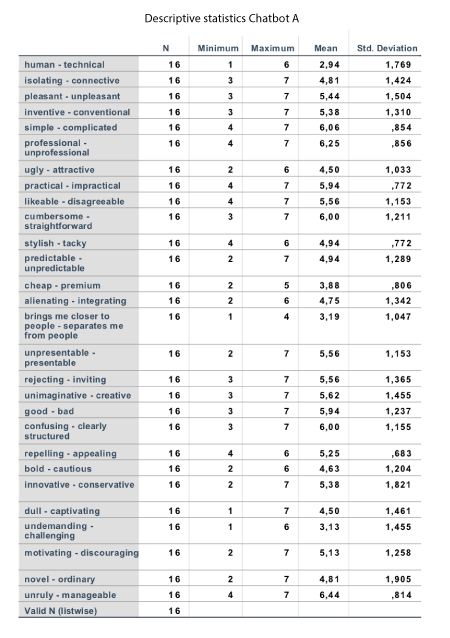
\includegraphics[scale=0.8]{figures/DescriptiveChatbotA.png}
        \caption{Descriptive statistics word pairs Chatbot A}
        \label{fig:deschatA}
    \end{figure}
    
    \begin{figure}[H]
        \centering
        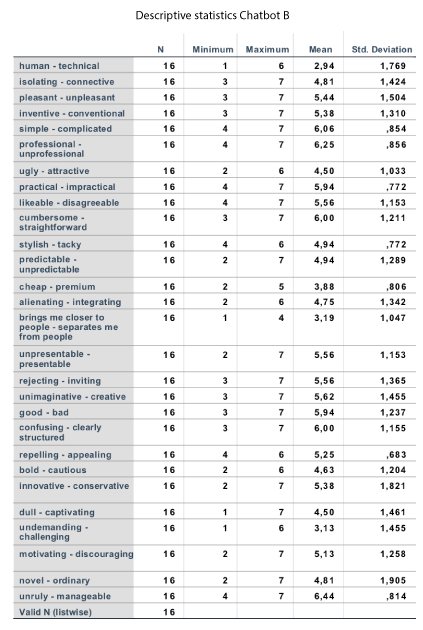
\includegraphics[scale=0.8]{figures/DescriptiveChatbotB.png}
        \caption{Descriptive statistics word pairs Chatbot B}
        \label{fig:deschatB}
    \end{figure}



%\include{inc/timetable}

\end{document}
